\documentclass[aspectratio=169,11pt]{beamer}
\usetheme{default}
\setbeamertemplate{navigation symbols}{}
\setbeamertemplate{footline}{%
  \hfill\insertframenumber/\inserttotalframenumber\hspace*{4pt}\vspace{2pt}%
}
\usepackage{lmodern}
\usepackage[most]{tcolorbox}
\usepackage{listings}
\usepackage{tikz}
\usetikzlibrary{arrows.meta,positioning,shapes.geometric,fit,backgrounds}
\usepackage{booktabs}
\usepackage{hyperref}

\definecolor{lcgreen}{HTML}{2E7D32}
\definecolor{lcblue}{HTML}{1565C0}
\definecolor{lcorange}{HTML}{EF6C00}
\definecolor{lcred}{HTML}{C62828}
\definecolor{codebg}{HTML}{F5F5F5}
\definecolor{docgray}{gray}{0.55}

\newtcolorbox{conceptbox}[1][]{colback=yellow!20,colframe=yellow!60!black,title=#1,fonttitle=\bfseries}
\newtcolorbox{warningbox}[1][]{colback=red!15,colframe=red!60!black,title=#1,fonttitle=\bfseries}
\newtcolorbox{tipbox}[1][]{colback=green!10,colframe=green!50!black,title=#1,fonttitle=\bfseries}
\newtcolorbox{codebox}[1][]{colback=blue!10,colframe=blue!40!black,title=#1,fonttitle=\bfseries}

\lstset{
  basicstyle=\ttfamily\scriptsize,
  backgroundcolor=\color{codebg},
  breaklines=true,
  frame=single,
  rulecolor=\color{blue!40!black},
  keywordstyle=\color{lcblue}\bfseries,
  stringstyle=\color{lcgreen},
  commentstyle=\color{docgray}\itshape,
  language=Python,
  showstringspaces=false,
  tabsize=2,
  xleftmargin=2pt,
  xrightmargin=2pt,
}

\newcommand{\docref}[1]{{\scriptsize\color{docgray}[Docs: #1]}}

\title{Document Loading \& Text Splitting}
\subtitle{LangChain v1.2.x --- Section 07}
\author{AI Engineering}
\date{March 2026}

\begin{document}

% Slide 1: Title
\begin{frame}
  \titlepage
\end{frame}

% Slide 2: Section Overview
\begin{frame}{Section Overview}
  \begin{itemize}
    \item \textbf{Why it matters:} Data ingestion is the foundation of RAG pipelines
    \item \textbf{Learning objectives:}
    \begin{itemize}
      \item Understand the Document ingestion pipeline
      \item Load documents from various sources
      \item Split documents intelligently for retrieval
      \item Manage metadata through the pipeline
    \end{itemize}
    \item \textbf{Scope:} LangChain v1.2.x (March 2026)
    \item \textbf{Slides:} 40 slides covering theory, code, and best practices
  \end{itemize}
\end{frame}

% Slide 3: Mental Model - Ingestion Pipeline
\begin{frame}{The Data Ingestion Pipeline}
  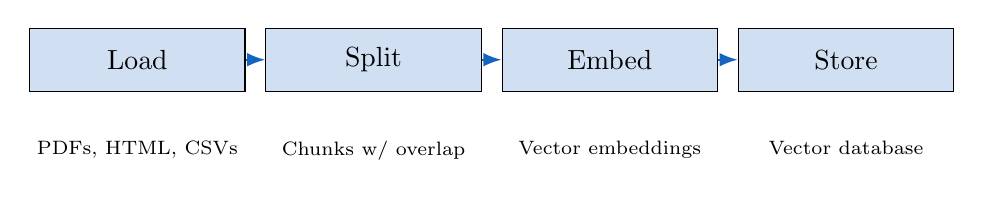
\begin{tikzpicture}[
    box/.style={rectangle, draw, fill=lcblue!20, text width=2.5cm, text centered, minimum height=0.8cm},
    arrow/.style={->,>=Latex,thick,lcblue}
  ]
    \node[box] (load) at (0, 0) {Load};
    \node[box] (split) at (3, 0) {Split};
    \node[box] (embed) at (6, 0) {Embed};
    \node[box] (store) at (9, 0) {Store};

    \draw[arrow] (load) -- (split);
    \draw[arrow] (split) -- (embed);
    \draw[arrow] (embed) -- (store);

    \node[below=0.5cm of load] {\scriptsize PDFs, HTML, CSVs};
    \node[below=0.5cm of split] {\scriptsize Chunks w/ overlap};
    \node[below=0.5cm of embed] {\scriptsize Vector embeddings};
    \node[below=0.5cm of store] {\scriptsize Vector database};
  \end{tikzpicture}

  \vspace{1.5cm}
  \begin{itemize}
    \item \textbf{Load:} Retrieve raw documents from various sources
    \item \textbf{Split:} Break documents into manageable chunks
    \item \textbf{Embed:} Convert text to vector representations
    \item \textbf{Store:} Index vectors for efficient retrieval
  \end{itemize}
\end{frame}

% Slide 4: The Document Object
\begin{frame}[fragile]{The Document Object}
  Core data structure in LangChain:
  \begin{lstlisting}
from langchain_core.documents import Document

doc = Document(
    page_content="Some text content",
    metadata={
        "source": "example.pdf",
        "page": 1,
        "author": "John Doe"
    }
)

print(doc.page_content)  # The actual text
print(doc.metadata)       # Dict of metadata
  \end{lstlisting}

  \vspace{0.5cm}
  \begin{conceptbox}{Key Aspects}
    \begin{itemize}
      \item \texttt{page\_content}: String containing the actual text
      \item \texttt{metadata}: Dictionary of arbitrary key-value pairs
      \item Metadata \textbf{must} be preserved through the pipeline for traceability
    \end{itemize}
  \end{conceptbox}
\end{frame}

% Slide 5: Document Loaders Interface
\begin{frame}[fragile]{Document Loaders --- Common Interface}
  All loaders inherit from \texttt{BaseLoader}:
  \begin{lstlisting}
from langchain_core.document_loaders import BaseLoader
from langchain_core.documents import Document
from typing import List

class BaseLoader(BaseModel):
    def load(self) -> List[Document]:
        """Load documents and return as list"""
        raise NotImplementedError

    def lazy_load(self) -> Iterator[Document]:
        """Stream documents one at a time"""
        raise NotImplementedError
  \end{lstlisting}

  \vspace{0.5cm}
  \begin{tipbox}{Two Load Modes}
    \begin{itemize}
      \item \texttt{load()}: Return all documents at once (for small datasets)
      \item \texttt{lazy\_load()}: Stream documents (for large datasets, memory efficient)
    \end{itemize}
  \end{tipbox}
\end{frame}

% Slide 6: TextLoader
\begin{frame}[fragile]{TextLoader --- Plain Text Files}
  Load simple text files:
  \begin{lstlisting}
from langchain_community.document_loaders import TextLoader

loader = TextLoader("document.txt")
documents = loader.load()

# For large files, stream instead:
for doc in loader.lazy_load():
    print(doc.page_content[:100])
  \end{lstlisting}

  \vspace{0.5cm}
  \begin{conceptbox}{Use Cases}
    \begin{itemize}
      \item .txt, .log, configuration files
      \item Source code files
      \item Simple documents without formatting
    \end{itemize}
  \end{conceptbox}

  \vspace{0.5cm}
  \textit{\docref{TextLoader: langchain/document\_loaders/text}}
\end{frame}

% Slide 7: PyPDFLoader
\begin{frame}[fragile]{PyPDFLoader --- PDF Documents}
  Extract text from PDF files with page tracking:
  \begin{lstlisting}
from langchain_community.document_loaders import PyPDFLoader

loader = PyPDFLoader("document.pdf")
documents = loader.load()

# Each page becomes a Document
for doc in documents:
    print(f"Page {doc.metadata['page']}: {doc.page_content[:100]}")
  \end{lstlisting}

  \vspace{0.5cm}
  \begin{itemize}
    \item Automatically extracts metadata (page number, file path)
    \item One \texttt{Document} per PDF page
    \item Preserves text structure from PDF
  \end{itemize}

  \textit{\docref{PyPDFLoader: langchain\_community/document\_loaders/pdf}}
\end{frame}

% Slide 8: CSVLoader
\begin{frame}[fragile]{CSVLoader --- Tabular Data}
  Load CSV files as documents:
  \begin{lstlisting}
from langchain_community.document_loaders.csv_loader import CSVLoader

loader = CSVLoader(
    file_path="data.csv",
    source_column="name"  # Which column is the source
)
documents = loader.load()

# Each row becomes a Document
for doc in documents:
    print(doc.page_content)
  \end{lstlisting}

  \vspace{0.5cm}
  \begin{itemize}
    \item Converts each CSV row to structured text
    \item Can specify which column contains the ``source''
    \item Useful for structured data like product catalogs
  \end{itemize}

  \textit{\docref{CSVLoader: langchain\_community/document\_loaders/csv}}
\end{frame}

% Slide 9: WebBaseLoader
\begin{frame}[fragile]{WebBaseLoader --- Web Pages}
  Scrape and load web pages:
  \begin{lstlisting}
from langchain_community.document_loaders import WebBaseLoader

urls = [
    "https://example.com/page1",
    "https://example.com/page2"
]
loader = WebBaseLoader(urls)
documents = loader.load()

for doc in documents:
    print(f"Source: {doc.metadata['source']}")
    print(f"Content: {doc.page_content[:100]}")
  \end{lstlisting}

  \vspace{0.5cm}
  \begin{itemize}
    \item Strips HTML, keeps text content
    \item Preserves source URL in metadata
    \item Great for knowledge base ingestion
  \end{itemize}

  \textit{\docref{WebBaseLoader: langchain\_community/document\_loaders/web}}
\end{frame}

% Slide 10: DirectoryLoader
\begin{frame}[fragile]{DirectoryLoader --- Batch File Loading}
  Load multiple files from a directory:
  \begin{lstlisting}
from langchain_community.document_loaders import DirectoryLoader

loader = DirectoryLoader(
    path="./documents/",
    glob="**/*.txt",  # Glob pattern for filtering
    loader_cls=TextLoader
)
documents = loader.load()
print(f"Loaded {len(documents)} documents")
  \end{lstlisting}

  \vspace{0.5cm}
  \begin{conceptbox}{Features}
    \begin{itemize}
      \item Use glob patterns to filter files
      \item Specify which loader class to use
      \item Supports recursive directory traversal (\texttt{**})
    \end{itemize}
  \end{conceptbox}

  \textit{\docref{DirectoryLoader: langchain\_community/document\_loaders/directory}}
\end{frame}

% Slide 11: Common Loaders Comparison Table
\begin{frame}{Document Loaders --- Comparison}
  \begin{center}
    \small
    \begin{tabular}{lcccc}
      \toprule
      \textbf{Loader} & \textbf{Source} & \textbf{Metadata} & \textbf{Streaming} & \textbf{Notes} \\
      \midrule
      TextLoader & .txt files & filename & Yes & Simple, fast \\
      PyPDFLoader & PDFs & page \#, path & Yes & Per-page split \\
      CSVLoader & CSV & row-based & Yes & Structured data \\
      WebBaseLoader & URLs & source URL & Yes & HTML stripping \\
      DirectoryLoader & Directory & per-file & Yes & Batch processing \\
      JSONLoader & JSON & custom & Yes & Structured \\
      MarkdownLoader & .md & path, heading & Yes & Code-friendly \\
      \bottomrule
    \end{tabular}
  \end{center}

  \vspace{1cm}
  \textit{All loaders support both \texttt{load()} and \texttt{lazy\_load()} modes}
\end{frame}

% Slide 12: Custom Loaders
\begin{frame}[fragile]{Custom Loaders --- Implementing BaseLoader}
  Create a custom loader for proprietary formats:
  \begin{lstlisting}
from langchain_core.document_loaders import BaseLoader
from langchain_core.documents import Document
from typing import List

class CustomLoader(BaseLoader):
    def __init__(self, file_path: str):
        self.file_path = file_path

    def load(self) -> List[Document]:
        with open(self.file_path, 'r') as f:
            content = f.read()
        return [Document(
            page_content=content,
            metadata={"source": self.file_path}
        )]
  \end{lstlisting}

  \vspace{0.5cm}
  Use: \texttt{docs = CustomLoader("data.custom").load()}
\end{frame}

% Slide 13: Why Text Splitting Matters
\begin{frame}{Why Text Splitting Matters}
  \begin{itemize}
    \item \textbf{Context windows are limited}: LLMs have finite token limits
    \begin{itemize}
      \item GPT-4: 8K, 32K, or 128K tokens
      \item Claude: 100K+ tokens
      \item Splitting ensures chunks fit in context
    \end{itemize}
    \item \textbf{Retrieval quality}: Small, focused chunks improve semantic search
    \item \textbf{Cost efficiency}: Pay for what you retrieve, not entire documents
    \item \textbf{Relevance}: Optimal chunk size balances specificity and context
  \end{itemize}

  \vspace{1cm}
  \begin{warningbox}{The Splitting Dilemma}
    Too small: Lose context. Too large: Exceed token limits or retrieve irrelevant content.
  \end{warningbox}
\end{frame}

% Slide 14: RecursiveCharacterTextSplitter
\begin{frame}[fragile]{RecursiveCharacterTextSplitter --- The Default}
  Most commonly used splitter in production:
  \begin{lstlisting}
from langchain_text_splitters import RecursiveCharacterTextSplitter

splitter = RecursiveCharacterTextSplitter(
    chunk_size=1000,        # Max characters per chunk
    chunk_overlap=200,      # Characters to overlap
    separators=[
        "\n\n",  # Paragraph
        "\n",    # Newline
        " ",     # Space
        ""       # Character fallback
    ]
)
chunks = splitter.split_documents(documents)
  \end{lstlisting}

  \vspace{0.5cm}
  \textit{\docref{RecursiveCharacterTextSplitter: langchain\_text\_splitters}}
\end{frame}

% Slide 15: How RecursiveCharacterTextSplitter Works
\begin{frame}{RecursiveCharacterTextSplitter --- Separator Hierarchy}
  Splits recursively using a hierarchy of separators:

  \begin{enumerate}
    \item Try splitting on \texttt{"\textbackslash n\textbackslash n"} (paragraphs)
    \item If chunks still too large, split on \texttt{"\textbackslash n"} (lines)
    \item If still too large, split on \texttt{" "} (words)
    \item If still too large, split on \texttt{""} (characters)
  \end{enumerate}

  \vspace{1cm}
  \begin{conceptbox}{Why Recursive?}
    \begin{itemize}
      \item Preserves semantic structure (paragraphs → lines → words)
      \item Better context preservation than naive splitting
      \item Handles documents with mixed formatting
    \end{itemize}
  \end{conceptbox}
\end{frame}

% Slide 16: Chunk Size and Overlap Tuning
\begin{frame}{Chunk Size and Overlap --- How to Choose}
  \vspace{0.3cm}
  \begin{itemize}
    \item \textbf{chunk\_size} (characters or tokens):
    \begin{itemize}
      \item Typical range: 512 to 2048 characters
      \item For dense docs: 500-800 chars (3-5 sentences)
      \item For sparse docs: 1000-2000 chars (longer context)
      \item Rule of thumb: about 1/4 of model's context window
    \end{itemize}

    \item \textbf{chunk\_overlap} (characters or tokens):
    \begin{itemize}
      \item Typical: 10-25 percent of chunk\_size
      \item Preserves context across chunk boundaries
      \item 200 overlap on 1000 chunk = 20 percent
      \item Too much overlap: redundant storage; too little: lost context
    \end{itemize}
  \end{itemize}

  \vspace{1cm}
  \begin{tipbox}{Tip}
    Start with chunk\_size=1000, overlap=200, then tune based on retrieval quality metrics.
  \end{tipbox}
\end{frame}

% Slide 17: Other Text Splitters
\begin{frame}[fragile]{Other Text Splitters}
  \begin{lstlisting}
# CharacterTextSplitter - simple, non-recursive
from langchain_text_splitters import CharacterTextSplitter
splitter = CharacterTextSplitter(chunk_size=1000, separator=" ")

# TokenTextSplitter - split by token count
from langchain_text_splitters import TokenTextSplitter
splitter = TokenTextSplitter(encoding_name="cl100k_base", chunk_size=100)

# MarkdownHeaderTextSplitter - preserve markdown structure
from langchain_text_splitters import MarkdownHeaderTextSplitter
splitter = MarkdownHeaderTextSplitter(
    headers_to_split_on=[("#", "Header 1"), ("##", "Header 2")]
)
chunks = splitter.split_text(markdown_string)
  \end{lstlisting}
\end{frame}

% Slide 18: Code Splitting
\begin{frame}[fragile]{Language-Aware Code Splitting}
  Split source code while preserving structure:
  \begin{lstlisting}
from langchain_text_splitters import Language, RecursiveCharacterTextSplitter

splitter = RecursiveCharacterTextSplitter.from_language(
    language=Language.PYTHON,
    chunk_size=1000,
    chunk_overlap=200
)

with open("script.py", "r") as f:
    code = f.read()

chunks = splitter.split_text(code)
  \end{lstlisting}

  \vspace{0.5cm}
  \begin{itemize}
    \item Supports: Python, JavaScript, TypeScript, Java, C++, Go, Rust, and more
    \item Uses language-specific separators (imports, class definitions, functions)
    \item Critical for code QA and documentation systems
  \end{itemize}
\end{frame}

% Slide 19: Metadata Management
\begin{frame}[fragile]{Preserving and Enriching Metadata}
  Metadata flows through the pipeline:
  \begin{lstlisting}
from langchain_community.document_loaders import PyPDFLoader
from langchain_text_splitters import RecursiveCharacterTextSplitter

loader = PyPDFLoader("doc.pdf")
docs = loader.load()  # Includes page metadata

splitter = RecursiveCharacterTextSplitter(chunk_size=1000)
chunks = splitter.split_documents(docs)  # Preserves metadata!

# Enrich metadata
for i, chunk in enumerate(chunks):
    chunk.metadata["chunk_id"] = i
    chunk.metadata["chunk_order"] = i

# Use in retrieval
for chunk in chunks:
    print(f"Source: {chunk.metadata['source']}, "
          f"Page: {chunk.metadata['page']}")
  \end{lstlisting}
\end{frame}

% Slide 20: Metadata Best Practices
\begin{frame}{Metadata Best Practices}
  \begin{itemize}
    \item \textbf{Always preserve original metadata:}
    \begin{itemize}
      \item Source file/URL
      \item Page/section number
      \item Author, timestamp
    \end{itemize}

    \item \textbf{Add processing metadata:}
    \begin{itemize}
      \item Chunk ID, chunk order
      \item Loader class name
      \item Processing timestamp
    \end{itemize}

    \item \textbf{Use for traceability:}
    \begin{itemize}
      \item Link retrieved chunks back to source
      \item Support citations in LLM responses
      \item Debug retrieval quality issues
    \end{itemize}
  \end{itemize}

  \vspace{0.5cm}
  \textbf{Rule:} Metadata must survive the entire pipeline: Load → Split → Embed → Store.
\end{frame}

% Slide 21: Document Processing Pipeline Diagram
\begin{frame}{Document Processing Pipeline --- Detailed View}
  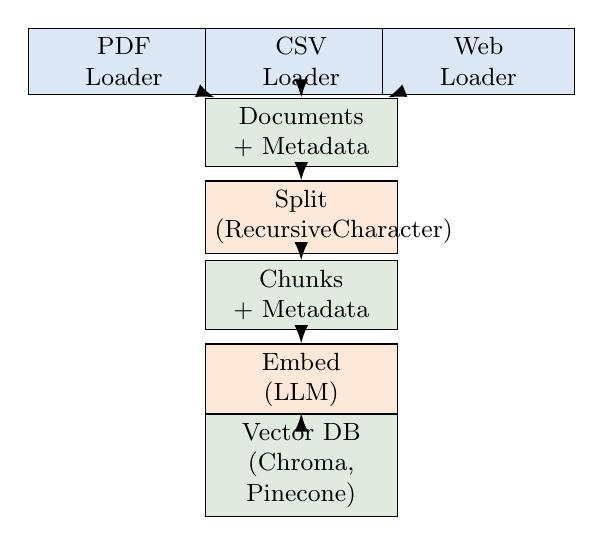
\begin{tikzpicture}[
    scale=0.9,
    box/.style={rectangle, draw, fill=lcblue!15, text width=2.2cm, text centered, minimum height=0.75cm, font=\small},
    process/.style={rectangle, draw, fill=lcorange!15, text width=2.2cm, text centered, minimum height=0.75cm, font=\small},
    storage/.style={rectangle, draw, fill=lcgreen!15, text width=2.2cm, text centered, minimum height=0.75cm, font=\small},
    arrow/.style={->,>=Latex,thick}
  ]
    % Row 1: Loading
    \node[box] (load1) at (0, 3) {PDF\\ Loader};
    \node[box] (load2) at (2.5, 3) {CSV\\ Loader};
    \node[box] (load3) at (5, 3) {Web\\ Loader};

    % Row 2: Documents
    \node[storage] (docs) at (2.5, 2) {Documents\\ + Metadata};
    \draw[arrow] (load1) -- (docs);
    \draw[arrow] (load2) -- (docs);
    \draw[arrow] (load3) -- (docs);

    % Row 3: Splitting
    \node[process] (split) at (2.5, 0.8) {Split\\(RecursiveCharacter)};
    \draw[arrow] (docs) -- (split);

    % Row 4: Chunks
    \node[storage] (chunks) at (2.5, -0.3) {Chunks\\+ Metadata};
    \draw[arrow] (split) -- (chunks);

    % Row 5: Embedding
    \node[process] (embed) at (2.5, -1.5) {Embed\\(LLM)};
    \draw[arrow] (chunks) -- (embed);

    % Row 6: Final Storage
    \node[storage] (store) at (2.5, -2.7) {Vector DB\\(Chroma, Pinecone)};
    \draw[arrow] (embed) -- (store);
  \end{tikzpicture}
\end{frame}

% Slide 22: Common Pitfall 1 - Wrong Chunk Size
\begin{frame}{Common Pitfall 1: Incorrect Chunk Size}
  \begin{center}
    \begin{tabular}{lll}
      \toprule
      \textbf{Chunk Size} & \textbf{Problem} & \textbf{Impact} \\
      \midrule
      Too small (< 200) & Lose context & Poor LLM responses \\
      Too large (> 4000) & Exceed token limits & API errors, cost \\
      Not tuned & Varies by document & Inconsistent quality \\
      \bottomrule
    \end{tabular}
  \end{center}

  \vspace{1cm}
  \begin{warningbox}{Solution}
    \begin{itemize}
      \item Estimate model's usable context: $0.25 \times \text{context\_window}$
      \item Start with default 1000, measure retrieval quality
      \item Use metrics: relevance score, response coherence, latency
    \end{itemize}
  \end{warningbox}
\end{frame}

% Slide 23: Common Pitfall 2 - Lost Metadata
\begin{frame}[fragile]{Common Pitfall 2: Losing Metadata}
  \begin{warningbox}{Danger}
    If metadata is lost during splitting, you cannot trace retrieved chunks back to source!
  \end{warningbox}

  \vspace{0.5cm}
  \begin{lstlisting}
# WRONG - metadata lost
chunks = splitter.split_text(text)  # str input, no metadata

# CORRECT - metadata preserved
docs = [Document(page_content=text, metadata={...})]
chunks = splitter.split_documents(docs)  # Document input
  \end{lstlisting}

  \vspace{0.5cm}
  \textbf{Always use:} \texttt{split\_documents()} with Document objects, not \texttt{split\_text()}.
\end{frame}

% Slide 24: Common Pitfall 3 - Encoding Issues
\begin{frame}[fragile]{Common Pitfall 3: Text Encoding Issues}
  \begin{warningbox}{Danger}
    PDFs and web pages may contain special characters, encodings that cause corruption.
  \end{warningbox}

  \vspace{0.5cm}
  \begin{lstlisting}
# Specify encoding when loading text files
from langchain_community.document_loaders import TextLoader

loader = TextLoader("document.txt", encoding="utf-8")
docs = loader.load()

# For PDFs, PyPDFLoader handles encoding automatically
# But test output for corrupted text
for doc in docs:
    if "\ufffd" in doc.page_content:  # Replacement char
        print("Warning: encoding error detected")
  \end{lstlisting}

  \vspace{0.5cm}
  \textbf{Tip:} Always inspect a sample of loaded documents for corruption.
\end{frame}

% Slide 25: Full Example - Load, Split, Store
\begin{frame}[fragile]{Full Example: Load → Split → Store}
  \small
  \begin{lstlisting}
from langchain_community.document_loaders import PyPDFLoader
from langchain_text_splitters import RecursiveCharacterTextSplitter
from langchain_openai import OpenAIEmbeddings
from langchain_community.vectorstores import Chroma

# Load
loader = PyPDFLoader("document.pdf")
docs = loader.load()

# Split
splitter = RecursiveCharacterTextSplitter(
    chunk_size=1000, chunk_overlap=200
)
chunks = splitter.split_documents(docs)

# Embed & Store
embeddings = OpenAIEmbeddings()
vectorstore = Chroma.from_documents(chunks, embeddings)

# Retrieve
results = vectorstore.similarity_search("query text", k=3)
  \end{lstlisting}
\end{frame}

% Slide 26: Handling Large Documents
\begin{frame}[fragile]{Handling Large Documents Efficiently}
  Use streaming (\texttt{lazy\_load}) for large files:
  \begin{lstlisting}
from langchain_community.document_loaders import PyPDFLoader
from langchain_text_splitters import RecursiveCharacterTextSplitter

loader = PyPDFLoader("huge_document.pdf")
splitter = RecursiveCharacterTextSplitter(
    chunk_size=1000, chunk_overlap=200
)

# Process one document at a time
for doc in loader.lazy_load():
    chunks = splitter.split_documents([doc])
    # Process/embed/store chunks immediately
    vectorstore.add_documents(chunks)
    # Don't accumulate in memory!
  \end{lstlisting}

  \vspace{0.5cm}
  \begin{itemize}
    \item Avoids loading entire document into memory
    \item Process and store in batches
    \item Critical for PDFs with hundreds of pages
  \end{itemize}
\end{frame}

% Slide 27: Batch Processing with DirectoryLoader
\begin{frame}[fragile]{Batch Processing Multiple Files}
  \begin{lstlisting}
from langchain_community.document_loaders import DirectoryLoader
from langchain_text_splitters import RecursiveCharacterTextSplitter
from langchain_community.vectorstores import Chroma
from langchain_openai import OpenAIEmbeddings

# Load all PDFs in directory
loader = DirectoryLoader(
    "documents/",
    glob="**/*.pdf",
    loader_cls=PyPDFLoader
)

# Split and embed
splitter = RecursiveCharacterTextSplitter(chunk_size=1000)
embeddings = OpenAIEmbeddings()
vectorstore = Chroma()

for doc in loader.lazy_load():
    chunks = splitter.split_documents([doc])
    vectorstore.add_documents(chunks)
  \end{lstlisting}
\end{frame}

% Slide 28: Token-Based Splitting
\begin{frame}[fragile]{Token-Based Splitting (More Accurate)}
  For precise control, split by token count instead of characters:
  \begin{lstlisting}
from langchain_text_splitters import TokenTextSplitter
from langchain.callbacks import get_openai_callback

# Split by tokens (more accurate than chars)
splitter = TokenTextSplitter(
    encoding_name="cl100k_base",  # GPT-4/3.5 encoding
    chunk_size=100,               # tokens
    chunk_overlap=20              # tokens
)

with get_openai_callback() as cb:
    chunks = splitter.split_documents(docs)
    print(f"Total tokens: {cb.total_tokens}")
  \end{lstlisting}

  \vspace{0.5cm}
  \textbf{Encoding names:}
  \begin{itemize}
    \item \texttt{cl100k\_base}: GPT-4, GPT-3.5-turbo
    \item \texttt{p50k\_base}: GPT-3
    \item \texttt{r50k\_base}: Text-davinci-003
  \end{itemize}
\end{frame}

% Slide 29: Advanced: Custom Metadata Extraction
\begin{frame}[fragile]{Advanced: Custom Metadata Extraction}
  Add smart metadata during processing:
  \begin{lstlisting}
from datetime import datetime
from langchain_community.document_loaders import PyPDFLoader
from langchain_text_splitters import RecursiveCharacterTextSplitter

loader = PyPDFLoader("document.pdf")
docs = loader.load()

splitter = RecursiveCharacterTextSplitter(chunk_size=1000)
chunks = splitter.split_documents(docs)

# Enrich with processing metadata
for i, chunk in enumerate(chunks):
    chunk.metadata.update({
        "chunk_sequence": i,
        "processed_at": datetime.now().isoformat(),
        "chunk_hash": hash(chunk.page_content) % (10**8),
        "character_count": len(chunk.page_content)
    })
  \end{lstlisting}
\end{frame}

% Slide 30: Debugging Document Processing
\begin{frame}[fragile]{Debugging Document Processing}
  \small
  \begin{lstlisting}
# Inspect loaded documents
docs = loader.load()
print(f"Loaded {len(docs)} documents")
for i, doc in enumerate(docs[:2]):
    print(f"Doc {i}: {len(doc.page_content)} chars")
    print(f"  Metadata: {doc.metadata}")

# Inspect chunks after splitting
chunks = splitter.split_documents(docs)
print(f"Created {len(chunks)} chunks")
for i, chunk in enumerate(chunks[:3]):
    print(f"Chunk {i}: {len(chunk.page_content)} chars, "
          f"tokens ~= {len(chunk.page_content) // 4}")
    print(f"  Preview: {chunk.page_content[:50]}...")

# Verify metadata preservation
if not all(chunks[0].metadata for chunk in chunks):
    print("WARNING: Some chunks missing metadata!")
  \end{lstlisting}
\end{frame}

% Slide 31: Performance Considerations
\begin{frame}{Performance Tuning}
  \begin{itemize}
    \item \textbf{Loading:}
    \begin{itemize}
      \item Use \texttt{lazy\_load()} for large files
      \item Batch processing with \texttt{DirectoryLoader}
    \end{itemize}

    \item \textbf{Splitting:}
    \begin{itemize}
      \item \texttt{RecursiveCharacterTextSplitter} is fast (CPU only)
      \item \texttt{TokenTextSplitter} slower (requires tokenizer)
      \item Larger overlap = more chunks (exponential storage cost)
    \end{itemize}

    \item \textbf{Embedding:}
    \begin{itemize}
      \item Batch API calls (embed multiple chunks at once)
      \item Cache embeddings to avoid recomputing
    \end{itemize}

    \item \textbf{Storage:}
    \begin{itemize}
      \item Use vector DB pagination for large collections
      \item Monitor memory usage with \texttt{lazy\_load()}
    \end{itemize}
  \end{itemize}
\end{frame}

% Slide 32: Special Cases - Markdown Documents
\begin{frame}[fragile]{Special Case: Markdown with Headers}
  Preserve document structure with markdown-aware splitting:
  \begin{lstlisting}
from langchain_text_splitters import MarkdownHeaderTextSplitter

markdown_splitter = MarkdownHeaderTextSplitter(
    headers_to_split_on=[
        ("#", "Header 1"),
        ("##", "Header 2"),
        ("###", "Header 3")
    ]
)

# Split markdown, preserving structure
chunks = markdown_splitter.split_text(markdown_content)

# Each chunk has header context in metadata
for chunk in chunks:
    print(f"Headers: {chunk.metadata}")
    print(f"Content: {chunk.page_content[:100]}")
  \end{lstlisting}
\end{frame}

% Slide 33: Special Cases - JSON and Structured Data
\begin{frame}[fragile]{Special Case: JSON Documents}
  Load and split structured JSON:
  \begin{lstlisting}
from langchain_community.document_loaders import JSONLoader
import json

# Load JSON file
loader = JSONLoader(
    file_path="data.json",
    jq_schema=".[]"  # Extract array elements
)
docs = loader.load()

# Split as usual
chunks = splitter.split_documents(docs)

# Each chunk is a JSON object as text
for chunk in chunks:
    print(chunk.page_content)
  \end{lstlisting}

  \vspace{0.5cm}
  \begin{itemize}
    \item Use \texttt{jq} syntax to extract relevant data
    \item Good for API responses, databases exported as JSON
  \end{itemize}
\end{frame}

% Slide 34: Cheat Sheet - Common Patterns
\begin{frame}[fragile]{Cheat Sheet: Common Patterns}
  \tiny
  \begin{lstlisting}
# 1. Simple PDF -> Chunks
docs = PyPDFLoader("file.pdf").load()
chunks = RecursiveCharacterTextSplitter(chunk_size=1000).split_documents(docs)

# 2. Directory of PDFs -> Chunks
loader = DirectoryLoader("pdfs/", glob="**/*.pdf", loader_cls=PyPDFLoader)
chunks = RecursiveCharacterTextSplitter(chunk_size=1000).split_documents(
    [doc for doc in loader.lazy_load()])

# 3. Multiple sources
from langchain_community.document_loaders import WebBaseLoader
urls_docs = WebBaseLoader(urls).load()
file_docs = TextLoader("file.txt").load()
all_docs = urls_docs + file_docs
chunks = RecursiveCharacterTextSplitter(chunk_size=1000).split_documents(all_docs)

# 4. Token-based splitting (precise)
chunks = TokenTextSplitter(encoding_name="cl100k_base", chunk_size=100).split_documents(docs)

# 5. Stream large files
for doc in PyPDFLoader("huge.pdf").lazy_load():
    chunks = RecursiveCharacterTextSplitter(chunk_size=1000).split_documents([doc])
    # Process/store immediately
  \end{lstlisting}
\end{frame}

% Slide 35: Self-Check Questions 1-3
\begin{frame}{Self-Check: Questions 1-3}
  \begin{enumerate}
    \item \textbf{Document Object:} What are the two main attributes of a LangChain \texttt{Document}? Why must metadata be preserved?

    \vspace{0.8cm}
    \item \textbf{Splitting Strategy:} Why does \texttt{RecursiveCharacterTextSplitter} work better than simple \texttt{CharacterTextSplitter}? Name the separator hierarchy.

    \vspace{0.8cm}
    \item \textbf{Chunk Size:} You're building a RAG system with GPT-4 (128K context). What chunk size would you start with and why? What's the relationship to token limits?
  \end{enumerate}
\end{frame}

% Slide 36: Self-Check Questions 4-6
\begin{frame}{Self-Check: Questions 4-6}
  \begin{enumerate}
    \setcounter{enumi}{3}
    \item \textbf{Loaders:} Describe the difference between \texttt{load()} and \texttt{lazy\_load()}. When would you use each?

    \vspace{0.8cm}
    \item \textbf{Metadata Pitfall:} What's the difference between \texttt{split\_text()} and \texttt{split\_documents()}? Which one preserves metadata?

    \vspace{0.8cm}
    \item \textbf{Large Files:} How would you process a 500-page PDF to avoid running out of memory? Describe the pipeline.
  \end{enumerate}
\end{frame}

% Slide 37: Self-Check Questions 7-8
\begin{frame}{Self-Check: Questions 7-8}
  \begin{enumerate}
    \setcounter{enumi}{6}
    \item \textbf{Token-Based Splitting:} Why might \texttt{TokenTextSplitter} be more accurate than character-based splitting? What encoding names do GPT-4 models use?

    \vspace{1.2cm}
    \item \textbf{Integration:} Write pseudocode for a complete pipeline: load PDFs from \texttt{./docs/} directory, split with overlap, embed, and store in a vector database.
  \end{enumerate}
\end{frame}

% Slide 38: Key Takeaways
\begin{frame}{Key Takeaways}
  \begin{itemize}
    \item \textbf{The pipeline matters:} Load → Split → Embed → Store are interdependent

    \item \textbf{Document object is sacred:} Always preserve metadata through all stages

    \item \textbf{RecursiveCharacterTextSplitter is the default:} Use it unless you have a specific reason not to

    \item \textbf{Chunk size affects everything:} Quality of retrieval, cost, speed --- experiment with metrics

    \item \textbf{Use lazy\_load() for production:} Stream processing avoids memory issues

    \item \textbf{Metadata = traceability:} Without it, you can't cite sources or debug failures
  \end{itemize}
\end{frame}

% Slide 39: Next Steps & Resources
\begin{frame}{Next Steps \& Resources}
  \begin{itemize}
    \item \textbf{Practice:}
    \begin{itemize}
      \item Load a PDF, split it, inspect chunks and metadata
      \item Experiment with chunk\_size and overlap values
      \item Build a small RAG prototype with your own documents
    \end{itemize}

    \item \textbf{Resources:}
    \begin{itemize}
      \item LangChain Docs: \texttt{python.langchain.com/docs/modules/data\_connection}
      \item Token counter: \texttt{platform.openai.com/tokenizer}
      \item OpenAI context limits: \texttt{platform.openai.com/docs/models}
    \end{itemize}

    \item \textbf{Advanced topics:}
    \begin{itemize}
      \item Semantic chunking (chunk by meaning, not size)
      \item Hybrid search (keyword + vector)
      \item Document hierarchy and parent-child retrieval
    \end{itemize}
  \end{itemize}
\end{frame}

% Slide 40: Summary Table
\begin{frame}{Summary: Quick Reference}
  \begin{center}
    \small
    \begin{tabular}{lll}
      \toprule
      \textbf{Task} & \textbf{Code Pattern} & \textbf{Key Parameter} \\
      \midrule
      Load PDF & \texttt{PyPDFLoader("file.pdf").load()} & Preserves page \# \\
      Load text & \texttt{TextLoader("file.txt").load()} & Simple, fast \\
      Load CSV & \texttt{CSVLoader("data.csv").load()} & source\_column \\
      Load web & \texttt{WebBaseLoader([urls]).load()} & Strips HTML \\
      Load dir & \texttt{DirectoryLoader("path", glob="**/*.pdf")} & Batch load \\
      Split (default) & \texttt{RecursiveCharacterTextSplitter()} & chunk\_size, overlap \\
      Split (tokens) & \texttt{TokenTextSplitter(chunk\_size=100)} & encoding\_name \\
      Debug & Print \texttt{len(docs)}, inspect \texttt{metadata} & Always verify \\
      \bottomrule
    \end{tabular}
  \end{center}
\end{frame}

% Slide 41: Thank You
\begin{frame}
  \centering
  \Huge\textbf{Questions?}

  \vspace{2cm}
  \Large Document Loading \& Text Splitting

  \vspace{1cm}
  \normalsize LangChain v1.2.x --- Section 07
\end{frame}

\end{document}
